%File Generated with PyPaper
\documentclass[aps,prl,reprint,amsmath,amssymb,superscriptaddress,notitlepage,groupedaddress]{revtex4-1}
\usepackage{graphicx}
\usepackage{dcolumn}
\usepackage{stackengine}
\usepackage[section]{placeins}
\usepackage[dvipsnames*,svgnames]{xcolor}
\usepackage{verbatim}
\usepackage[position=bottom,caption=false,captionskip=3pt,font=normalsize,subrefformat=simple,labelformat=simple]{subfig}
\renewcommand{\thesubfigure}{(\alph{subfigure})}
\usepackage{listings}
\usepackage{mathtools}
\usepackage{todonotes}
\usepackage{amsmath}
\usepackage{chngcntr}
\usepackage{bm}
\usepackage{url}
\def\UrlBreaks{\do\/\do-}
\newcommand {\framedgraphic}[2] {\begin{frame}{#1}\begin{center}\includegraphics[width=\textwidth,height=0.8\textheight,keepaspectratio]{#2}\end{center}\end{frame}}\usepackage[breaklinks]{hyperref}
\usepackage{breakurl}
\usepackage{tabularx}
\usepackage{soul}
\hypersetup{
colorlinks,
linkcolor={blue!100!black},
citecolor={blue},
urlcolor={blue!80!black}}
\lstset{basicstyle=\small\ttfamily,columns=flexible,breaklines=true}\newcommand{\fakesection}[1]{\par\refstepcounter{section}\sectionmark{#1}\addcontentsline{toc}{section}{\protect\numberline{\thesection}#1}}\def\equationautorefname~#1\null{#1\null}
\raggedbottom\usepackage[bottom]{footmisc} \makeatletter \def\p@section{} \def\p@subsubsection{} \makeatother\begin{document}
\title{Bayesim: a tool for fast device characterization with Bayesian inference}
\author{Rachel Kurchin}
\affiliation{Department of Mechanical Engineering, Massachusetts Institute of Technology, 77 Massachusetts Avenue, Cambridge, MA 02139, USA}
\author{Giuseppe Romano}
\affiliation{Department of Mechanical Engineering, Massachusetts Institute of Technology, 77 Massachusetts Avenue, Cambridge, MA 02139, USA}
\author{Tonio Buonassisi}
\email{buonassi@mit.edu}
\affiliation{Department of Mechanical Engineering, Massachusetts Institute of Technology, 77 Massachusetts Avenue, Cambridge, MA 02139, USA}
\begin{abstract}
Target journal: Computer Physics Communications\end{abstract}
\maketitle

\fakesection{fake}
 
\section*{Introduction}
 motivation (within PV and beyond) citing examples of our application of this idea so far (Joule paper and PVSC proceeding) 
\section*{Model}
 \begin{itemize}
 \item background on Bayes theorem
 \item particulars about how it can be applied to fitting problems we're interested in
 \item advantages over traditional fitting approaches
 \item figure 1
 \end{itemize}
  
\begin{figure}[!ht]

\subfloat[\label{Fig:10a}]
{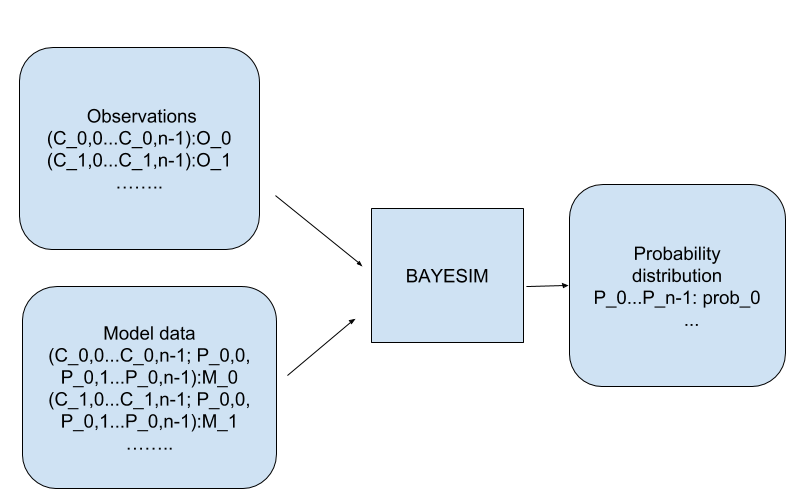
\includegraphics[width=0.48\columnwidth]{././figure_1a.png}}
\hfill
\subfloat[\label{Fig:10b}]
{
\includegraphics[width=0.48\columnwidth]{././figure_1b.png}}
\caption{(a) Scheme (b) Probability}
\end{figure}

\section*{Software Architecture and Interface}
 \begin{itemize}\item description of structure of new code and workflow for using it (both Python scripting and command-line) \item figure 2 \end{itemize}  \begin{figure}
{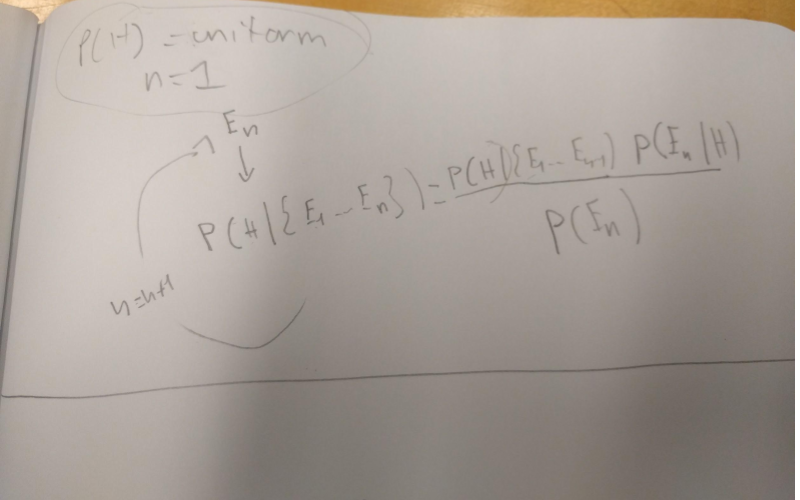
\includegraphics[width=0.7\columnwidth]{././figure_2.png}}
\caption{Bayesian workflow}
\end{figure}
\section*{Application Examples}
 \subsection{Ideal Diode Model}
  \begin{itemize}\item validation example - ``observed'' data is just generated using the model and we show we can recover the correct input parameters \item figure 3 showing PMF (animation in ESI) \end{itemize}  \begin{figure}
{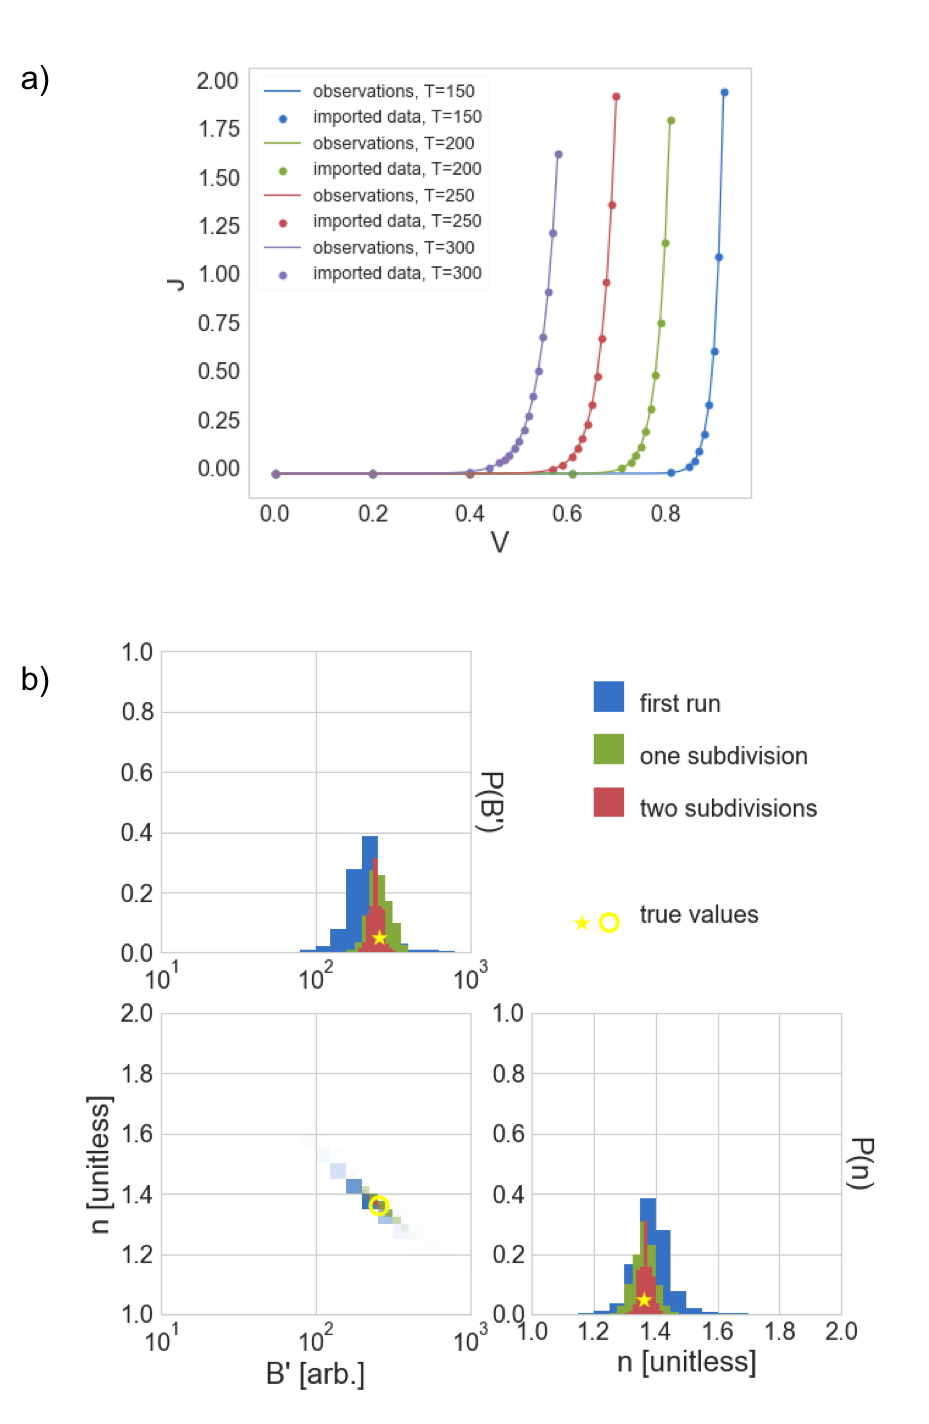
\includegraphics[width=0.7\columnwidth]{././figure_3.png}}
\caption{Ideal diode}
\end{figure}\subsection{Example with Real Data}
  \begin{itemize}\item more practical example - probably fitting resistive diode to the same SnS data we used in the Joule paper \item figure 4 showing PMF (animation in ESI) and comparison of JV curves \end{itemize} \todo[inline]{example fgryer2qt rt r}  
\begin{figure}[!ht]

\subfloat[\label{Fig:40a}]
{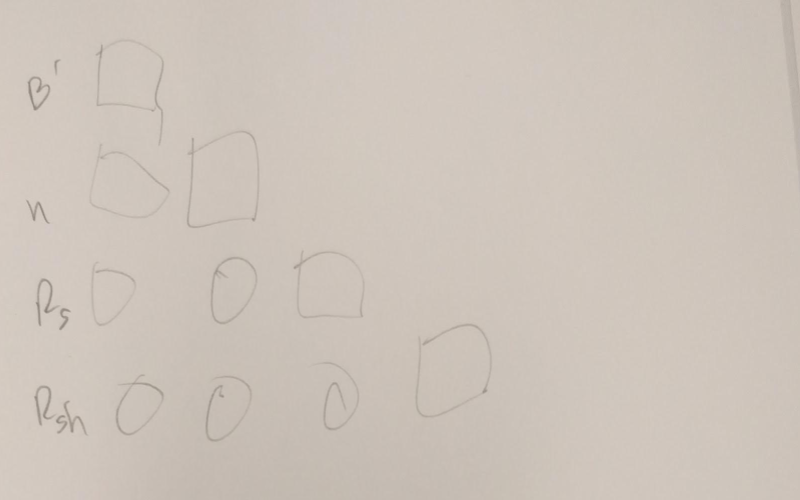
\includegraphics[width=0.48\columnwidth]{././figure_4a.png}}
\hfill
\subfloat[\label{Fig:40b}]
{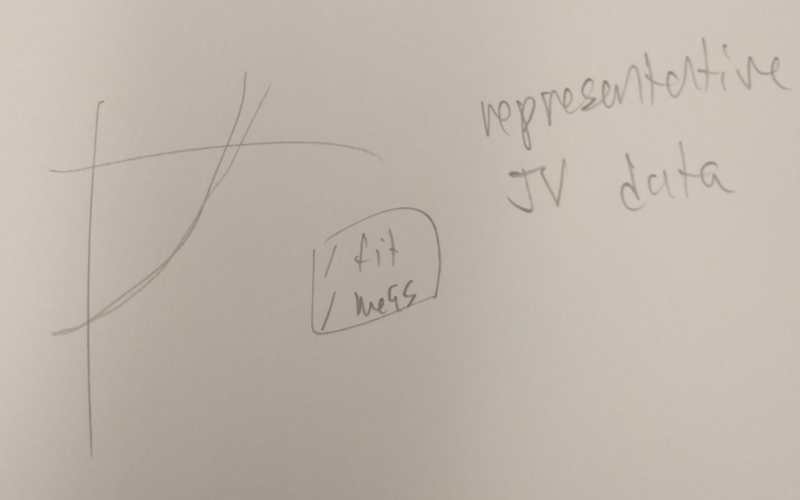
\includegraphics[width=0.48\columnwidth]{././figure_4b.png}}
\caption{Real data}
\end{figure}
\subsection{Maybe an example with a numerical model like PC1D}
  \subsection{Maybe a non-PV example}
  thermoelectrics? TIDLS? 
\section*{Conclusions}
 
\section*{Acknowledgements}
 
\section*{Appendix}
 \begin{itemize}\item include minimal code to run ideal diode example \item link to Github repo (which has installation instructions and documentation as well as list of planned future features) \end{itemize} %merlin.mbs apsrev4-1.bst 2010-07-25 4.21a (PWD, AO, DPC) hacked
%Control: key (0)
%Control: author (8) initials jnrlst
%Control: editor formatted (1) identically to author
%Control: production of article title (-1) disabled
%Control: page (0) single
%Control: year (1) truncated
%Control: production of eprint (0) enabled
\begin{thebibliography}{0}%
\makeatletter
\providecommand \@ifxundefined [1]{%
 \@ifx{#1\undefined}
}%
\providecommand \@ifnum [1]{%
 \ifnum #1\expandafter \@firstoftwo
 \else \expandafter \@secondoftwo
 \fi
}%
\providecommand \@ifx [1]{%
 \ifx #1\expandafter \@firstoftwo
 \else \expandafter \@secondoftwo
 \fi
}%
\providecommand \natexlab [1]{#1}%
\providecommand \enquote  [1]{``#1''}%
\providecommand \bibnamefont  [1]{#1}%
\providecommand \bibfnamefont [1]{#1}%
\providecommand \citenamefont [1]{#1}%
\providecommand \href@noop [0]{\@secondoftwo}%
\providecommand \href [0]{\begingroup \@sanitize@url \@href}%
\providecommand \@href[1]{\@@startlink{#1}\@@href}%
\providecommand \@@href[1]{\endgroup#1\@@endlink}%
\providecommand \@sanitize@url [0]{\catcode `\\12\catcode `\$12\catcode
  `\&12\catcode `\#12\catcode `\^12\catcode `\_12\catcode `\%12\relax}%
\providecommand \@@startlink[1]{}%
\providecommand \@@endlink[0]{}%
\providecommand \url  [0]{\begingroup\@sanitize@url \@url }%
\providecommand \@url [1]{\endgroup\@href {#1}{\urlprefix }}%
\providecommand \urlprefix  [0]{URL }%
\providecommand \Eprint [0]{\href }%
\providecommand \doibase [0]{http://dx.doi.org/}%
\providecommand \selectlanguage [0]{\@gobble}%
\providecommand \bibinfo  [0]{\@secondoftwo}%
\providecommand \bibfield  [0]{\@secondoftwo}%
\providecommand \translation [1]{[#1]}%
\providecommand \BibitemOpen [0]{}%
\providecommand \bibitemStop [0]{}%
\providecommand \bibitemNoStop [0]{.\EOS\space}%
\providecommand \EOS [0]{\spacefactor3000\relax}%
\providecommand \BibitemShut  [1]{\csname bibitem#1\endcsname}%
\let\auto@bib@innerbib\@empty
%</preamble>
\end{thebibliography}%
\end{document}
